% !TeX root = ../master.tex

\lecture{6}{2026-09-10}{Makromekanik af Lamina, Pt. I}

\section{Makromekanik}

\subsection{Makromekanik for Anisotropiske Lamina}
Makromekanik for et-lags kompositter, \textit{Lamina}, vil i dette afsnit gennemgås.
Makromekanik bekymrer sig ikke om fibre eller matrixmaterialerne i sig selv, men ser i stedet laminaen som bestående af et homogent materiale.

\subsubsection{Stivheds- og Compliancematricen}
Vi har spændings-tøjningsrelationen:
\begin{equation*}
  \sigma_i = C_{ij} \epsilon_j, \qquad i, j = 1,\ldots 6
.\end{equation*}
Altså er stivhedsmatricen $C$ en matrix med 36 værdier.
Stivhedsmatricen kan dog reduceres til 21 unikke værdier grundet symmetri, $C_{ij} = C_{ji}$ -- dette gælder også i anisotrope materialer.

Compliance matrixen $S$ er stivhedsmatricen $C$'s inverse:
\begin{equation*}
  S = C^{-1}
\end{equation*}
hvorfor spændings-tøjningsrelationene også kan skrives som
\begin{equation*}
  \epsilon_i = S_{ij} \sigma_j, \qquad i,j = 1,\ldots ,6
\end{equation*}
Compliancematrixen kan også reduceres til 21 unikke værdier grundet symmetri, $S_{ij} = S_{ji}$

\subsubsection{Koblingseffekter}
Copmliancematricen tydeliggør en række koblingseffekter mellem tøjninger og spændinger i 3-D, se \Mref{fig:coupling}.

\begin{figure} [ht]
  \centering
  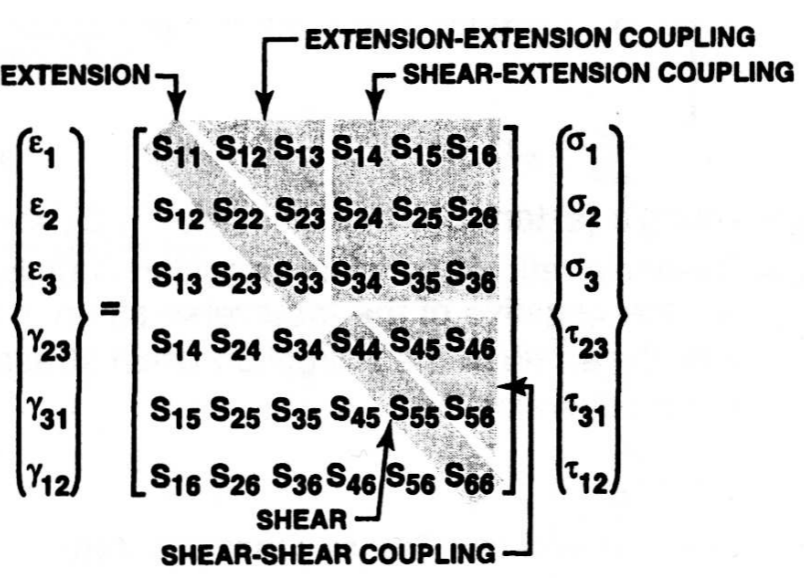
\includegraphics[width=0.65\linewidth]{./figures/coupling.png}
  \caption{Koblingseffekter fra Compliancematrixen, \citepage{jones2021mechanicscompositematerials}{fig. 2--5}.}
  \label{fig:coupling}
\end{figure}

\subsection{Makromekanik for Isotropiske Lamina}
For isotropiske materialer simplificeres spændings-tøjningsrelationen til
\begin{equation*}
  \begin{bmatrix}
    \epsilon_1\\
  \epsilon_2\\
  \epsilon_3\\
  \gamma_{23}\\
  \gamma_{31}\\
  \gamma_{12}\\
  \end{bmatrix} = \begin{bmatrix}
    S_{11} & S_{12} & S_{12} & 0 & 0 & 0\\
  S_{12} & S_{11} & S_{12} & 0 & 0 & 0\\
  S_{12} & S_{12} & S_{11} & 0 & 0 & 0\\
  0 & 0 & 0 & 2 \left( S_{11} - S_{12} \right) & 0 & 0\\
  0 & 0 & 0 & 0 & 2 \left( S_{11} - S_{12} \right) & 0\\
  0 & 0 & 0 & 0 & 0 & 2 \left( S_{11} - S_{12} \right) \begin{bmatrix}
    \sigma_1\\
  \sigma_2\\
  \sigma_3\\
  \tau_{23}\\
  \tau_{31}\\
  \tau_{12}\\
  \end{bmatrix}\\
  \end{bmatrix}
.\end{equation*}
Heri kan bemærkes at $S_{11} = E$ og $S_{12} = \nu$.

\subsection{Makromekanik for Ortotropiske Lamina}
For et ortotropisk materiale bliver spændings-tøjningsrelationen:
\begin{equation*}
  \begin{bmatrix}
    \epsilon_1\\
  \epsilon_2\\
  \epsilon_3\\
  \gamma_{23}\\
  \gamma_{31}\\
  \gamma_{12}\\
  \end{bmatrix} = \begin{bmatrix}
    S_{11} & S_{12} & S_{13} & 0 & 0 & 0\\
  S_{12} & S_{22} & S_{23} & 0 & 0 & 0\\
  S_{13} & S_{23} & S_{33} & 0 & 0 & 0\\
  0 & 0 & 0 & S_{44} & 0 & 0\\
  0 & 0 & 0 & 0 & S_{55} & 0\\
  0 & 0 & 0 & 0 & 0 & S_{66} \begin{bmatrix}
    \sigma_1\\
  \sigma_2\\
  \sigma_3\\
  \tau_{23}\\
  \tau_{31}\\
  \tau_{12}\\
  \end{bmatrix}\\
  \end{bmatrix}
.\end{equation*}
Compliancematrixen her kan også skrives med udgangspunkt i materialekonstanter:
\begin{equation*}
  S = \begin{bmatrix}
    \frac{1}{E_1} & - \frac{\nu_{21}}{E_2} & - \frac{\nu_{31}}{E_3} & 0 & 0 & 0\\
  - \frac{\nu_{12}}{E_1} & \frac{1}{E_2} & - \frac{\nu_{32}}{E_3} & 0 & 0 & 0\\
  - \frac{\nu_{13}}{E_1} & - \frac{\nu_{23}}{E_2} & \frac{1}{E_3} & 0 & 0 & 0\\
  0 & 0 & 0 & 0 & \frac{1}{G_{23}} & 0\\
  0 & 0 & 0 & 0 & \frac{1}{G_{13}} & 0\\
  0 & 0 & 0 & 0 & 0 & \frac{1}{G_{12}}\\
  \end{bmatrix}
.\end{equation*}
Idet compliancematrixen er symmetrisk har vi at:
\begin{equation*}
  \frac{\nu_{ij}}{E_i} = \frac{\nu_{ji}}{E_j}
\end{equation*}
altså er $\nu_{12} \neq \nu_{21}$

\subsection{Materialekonstanter}

\subsubsection{Isotropiske Materialer}
Shear og bulk modulus for isotropiske materialer er:
\begin{align*}
  G &= \frac{E}{2 \left( 1 + \nu \right)} \\
  K &= \frac{E}{3 \left( 1 - 2\nu \right)}
\end{align*}
og Poissons forhold er tvunget
\begin{equation*}
  -1 < \nu < \frac{1}{2}
.\end{equation*}

\subsubsection{Ortotropiske Materialer}
For ortotropiske materialer er $S_{ii} > 0$ og $C_{ii} > 0$, hvilket fører til følgende restriktioner for Poissons forhold
\begin{align*}
  1 - \nu_{23} \nu_{32} &> 0 \\
  1 - \nu_{13} \nu_{31} &>0 \\
  1 - \nu_{12}\nu_{31} &> 0 \\
  1 - \nu_{12}\nu_{21} - \nu_{23}\nu_{32} - \nu_{31}\nu_{13} - 2\nu_{21}\nu_{32}\nu_{13} &> 0
.\end{align*}
Ved introduktion af den reciprokke relation har vi:
\begin{align*}
  \left| \nu_{12} \right| &< \sqrt{\frac{E_1}{E_2}} \\
  \left| \nu_{23} \right| &< \sqrt{\frac{E_2}{E_3}} \\
  \left| \nu_{13} \right| &< \sqrt{\frac{E_1}{E_3}} \\
  \left| \nu_{21} \right| &< \sqrt{\frac{E_2}{E_1}} \\
  \left| \nu_{32} \right| &< \sqrt{\frac{E_3}{E_2}} \\
  \left| \nu_{31} \right| &< \sqrt{\frac{E_3}{E_1}}
.\end{align*}

\subsection{Planspænding}
En spænding kan siges at ligge i et plan når
\begin{equation*}
  \sigma_3 = \tau_{13} = \tau_{23} = 0
.\end{equation*}
Dette er en gyldig antagelse når tykkelsen, $t$ er lille i forhold til længden eller bredden $W$.
Den generelle tommelfingerregel er:
\begin{equation*}
  \frac{t}{W} \leq \num{0,1} 
.\end{equation*}
Altså er planspænding brugbart for skaller (her bruges krumningsradius dog som $t$) og tynde plader.

For planspænding er $\sigma_3 = \tau_{23} = \tau_{13} = 0$, hvorfor spændings-tøjningsrelationen kan reduceres til
\begin{equation} \label{eq:planspænding}
  \begin{bmatrix}
    \sigma_1\\
  \sigma_2\\
  \tau_{12}\\
  \end{bmatrix} = \begin{bmatrix}
    Q_{11} & Q_{12} & 0\\
  Q_{12} & Q_{22} & 0\\
  0 & 0 & Q_{66}\\
  \end{bmatrix} \begin{bmatrix}
    \epsilon_1\\
  \epsilon_2\\
  \gamma_{12}\\
  \end{bmatrix}
.\end{equation}
I \Mref{eq:planspænding} introduceredes den reducerede stivhedsmatrice $Q$, hvor indgangene er givet fra materialekonstanter efter:
\begin{align*}
  Q_{11} &= \frac{E_1}{1 - \nu_{12} \nu_{21}} \\
  Q_{22} &= \frac{E_2}{1 - \nu_{12} \nu_{21}} \\
  Q_{12} &= \frac{\nu_{21}E_1}{1 - \nu_{12}\nu_{21}} = \frac{\nu_{12} E_2}{1 - \nu_{12}\nu_{21}} \\
  Q_{66} &= Q_{12}
.\end{align*}
